\documentclass[12pt]{ucthesis}

\usepackage{etex}
\usepackage[morefloats=125]{morefloats}
\usepackage[hyphens]{url}
\usepackage{subfig}
\usepackage{graphicx}
\usepackage{tabularx}
\usepackage{amssymb}
\usepackage{amsmath}
\usepackage[letterpaper]{geometry}
\usepackage[overload]{textcase}
\usepackage[nonumberlist,toc]{glossaries}
\usepackage{wrapfig}
\usepackage{longtable}
\usepackage{morefloats}
\usepackage{float}
\usepackage{listings}
\usepackage{color}
\usepackage{colortbl}
 
\definecolor{codegreen}{rgb}{0,0.6,0}
\definecolor{codegray}{rgb}{0.5,0.5,0.5}
\definecolor{codepurple}{rgb}{0.58,0,0.82}
\definecolor{backcolour}{rgb}{0.95,0.95,0.92}

\definecolor{tablegreen}{rgb}{0.9, 1.0, 0.9}
\definecolor{tablered}{rgb}{1.0, 0.9, 0.9}

\usepackage{courier}
 
\lstdefinestyle{mystyle}{
    backgroundcolor=\color{backcolour},   
    commentstyle=\color{codegreen},
    keywordstyle=\color{magenta},
    numberstyle=\tiny\color{codegray},
    stringstyle=\color{codepurple},
    basicstyle=\footnotesize\ttfamily,
    breakatwhitespace=false,         
    breaklines=true,                 
    captionpos=b,                    
    keepspaces=true,                 
    numbers=left,                    
    numbersep=5pt,                  
    showspaces=false,                
    showstringspaces=false,
    showtabs=false,                  
    tabsize=2,
    frame=single
}
 
\lstset{
	style=mystyle,
	breakatwhitespace,
}

\usepackage{makecell}
\usepackage{appendix}
\usepackage[]{algorithm2e}
\usepackage{titlesec}
\usepackage{tikz}
\usetikzlibrary{arrows}
\usetikzlibrary{shapes}
\usetikzlibrary{patterns}
\usepackage[breaklinks=true,hidelinks,pdfusetitle]{hyperref}
\usepackage{cleveref}
\usepackage{ifthen}

\makeindex
\makeglossaries

% Shrink the size of headers
\titleformat{\chapter}[display]
        {\normalfont\normalsize\centering}
        {\ifthenelse{\equal{\thechapter}{A}}{APPENDICES\\[4.3ex]}{}\chaptertitlename\ \thechapter}
        {0pt}{\normalsize\uppercase}
\titlespacing*{\chapter}{0pt}{-20pt}{4.3ex plus .2ex}


\titleformat{\section}[block]{\normalsize\bfseries}{\thesection. }{}{}
\titleformat{\subsection}[block]{\small\bfseries}{\thesubsection. }{}{}
\titleformat{\subsubsection}[block]{\small\bfseries}{\thesubsubsection. }{}{}
\titleformat{\paragraph}[block]{\small\bfseries}{}{}{}
\titleformat{\subparagraph}[block]{\small\bfseries}{}{}{}

\bibliographystyle{abbrv}

\setlength{\parindent}{0.25in} \setlength{\parskip}{6pt}
\geometry{verbose,nohead,tmargin=1in,bmargin=1in,lmargin=1.5in,rmargin=1in}
\setcounter{tocdepth}{2}

% Different font in captions (single-spaced, bold) ------------
\newcommand{\captionfonts}{\small\bf\ssp}

\newcommand{\mycaption}[2]{\caption[#1 --- #2]{#1 --- #2}}

\makeatletter  % Allow the use of @ in command names
\long\def\@makecaption#1#2{%
  \vskip\abovecaptionskip
  \sbox\@tempboxa{{\captionfonts #1: #2}}%
  \ifdim \wd\@tempboxa >\hsize
    {\captionfonts #1: #2\par}
  \else
    \hbox to\hsize{\hfil\box\@tempboxa\hfil}%
  \fi
  \vskip\belowcaptionskip}
\makeatother   % Cancel the effect of \makeatletter
% ---------------------------------------

% Define Appendix refs
\crefname{app}{appendix}{appendices}
\Crefname{app}{Appendix}{Appendices}


\makeatletter
\renewcommand\lstlistoflistings{%
	\newpage
    \if@twocolumn
      \@restonecoltrue\onecolumn
    \else
      \@restonecolfalse
    \fi
    \addcontentsline{toc}{chapter}{LIST OF LISTINGS}
    \begin{center}
      \MakeUppercase{List of Listings} \\[1.5ex]
     % CHAPTER \hfill{} PAGE
    \end{center}

	Listing \hfill Page

    %\chapter*{\contentsname
    %    \@mkboth{%
    %       \MakeUppercase\contentsname}{\MakeUppercase\contentsname}}%
    \@starttoc{lol}%
    \if@restonecol\twocolumn\fi
    }
\makeatother

\begin{document}

% Declarations for Front Matter
\title{Funqual: User-Defined, Statically-Checked Call-Tree Constraints in C++}
\author{Andrew Nelson}
\degreemonth{June} \degreeyear{2018} \degree{Master of Science}
\defensemonth{June} \defenseyear{2018}
\numberofmembers{2}
   \chair{Aaron Keen, Ph.D. \linebreak Professor of Computer Science}
   \othermemberA{John Clements, Ph.D. \linebreak Professor of Computer Science}
   \othermemberB{Phillip Nico, Ph.D. \linebreak Professor of Computer Science}
\field{Computer Science} \campus{San Luis Obispo}
\copyrightyears{seven}


\maketitle

\begin{frontmatter}

% Custom made for Cal Poly (by Mark Barry, modified by Andrew Tsui).
\copyrightpage

% Custom made for Cal Poly (by Andrew Tsui).
\committeemembershippage

\begin{abstract}
Static analysis tools can aid programmers by reporting potential programming mistakes prior to the execution of a program.  Funqual is a static analysis tool that reads C++17 code ``in the wild'' and checks that the function call graph follows a set of rules which can be defined by the user.  This sort of analysis can help the programmer to avoid errors such as accidentally calling blocking functions in time-sensitive contexts or accidentally allocating memory in heap-sensitive environments.  To accomplish this, we create a type system whereby functions can be given user-defined type qualifiers and where users can define their own restrictions on the call tree based on these type qualifiers.  We demonstrate that this tool, when used with hand-crafted rules, can catch certain types of errors which commonly occur in the wild.  We claim that this tool can be used in a production setting to catch certain kinds of errors in code before that code is even run.  


\end{abstract}

\begin{acknowledgements}
\noindent
Thanks to:
\begin{itemize}
    \item Dennis Ritchie and Bjarne Stroustrup.  You've accidentally created something hauntingly expressive, painstakingly verbose, ingeniously strict, and idiotically sloppy.  C++17 is a hot mess but it's everywhere --- thank God it's type safe.  
\end{itemize}

\end{acknowledgements}

\tableofcontents

\listoftables

\listoffigures

\lstlistoflistings

% Add CHAPTER into table of contents.
\addtocontents{toc}{%
   \noindent CHAPTER
}

\end{frontmatter}

\pagestyle{plain}

\renewcommand{\baselinestretch}{1.66}


%\chapter{Introduction}

Writing bug-free software is challenging if not impossible.  In the past 30 years, millions of dollars have been invested in tools that help developers write code that is robust, readable, and correct \cite{staticanal}.  In general these tools fall into two categories:  Dynamic Analysis tools such as gdb, valgrind, and IDA which analyze programs as they are running; and Static Analysis tools such as lint, cppcheck, and GCC -WAll.  All these tools have different use cases and can be used in conjunction to write code that is error-free.

Languages like C++ and java are well suited for static analysis because type information is explicit in the source code and because every identifier must have one singular unambiguous type.  This enables static analysis tools to do a great deal of checking before even running the program.  

The following snippet of C++ code demonstrates this concept:

\begin{lstlisting}[language=C]
    int i = 2 + false;
\end{lstlisting}

The error here is trivial and easy for a human to spot by simple inspection.  However, as code gets more complex and as codebases get larger, errors like this can be hidden by layers of abstraction.  A tool like GCC or cppcheck is able to spot an error like this nearly instantaneously from the perspective of the programmer and is able to do it for massive codebases.  When using a language like python or ruby, an error like this might not be detected until the code is executed which could take minutes or months.  It is clear to see how being able to detect errors like this statically provides great benefit to the programmer.  A classic study by the University of North Carolina in conjunction with Nortel Networks found that the use of automated static analysis can detect certain types of programming errors at approximately the same accuracy as manual code inspection and that this checking can be performed in a fraction of the time \cite{staticanal}.  

In recent years there has been a big push to expand the realm of what can be statically checked.  A very successful example would be the Rust programming language from Mozilla which was designed to provide "strong guarantees about isolation, concurrency, and memory safety" using an innovate set of type annotations and static analysis techniques \cite{rust-is-dope}. 

Interestingly, before the advent of the Rust project, Mozilla had a fairly lengthy relationship with statically checking for some of these things in C++ code using their Pork tool \cite{mozilla-pork, mozilla-pork-blog}.  Using Pork, Mozilla developed a fairly robust set of tooling aimed at using static analysis to detect certain memory issues and API mis-uses in C++ code used in Mozilla projects.  While these tools were never able to do exhaustive program-wide checking, they were able to check a fair number of commonly-occurring issues.  

Of course, there are things which are extremely difficult to statically check in C and C++.  For years, various projects have tried to build tools which can statically analyze code to check for memory errors, unit errors, and infinite loops.  Unfortunately, many of these projects require specific language extensions in order for there to be enough information in the source code for the tools to work.  This is unfortunate because it prevents the tools from being used on code "in the wild", or code that has not been written with the tool in mind.

This thesis explores static analysis of a program's call-graph.  Specifically, we create a tool called funqual which allows C++ programmers to tag certain functions as belonging to certain types and which can statically check the call-graph and function types against a set of user-defined rules.  This call-graph type system is totally orthogonal to the existing C++ typesystem and so does not interfere with or expand the existing type rules which should be familiar to C++ programmers.  Instead, funqual provides an additional set of restrictions which, when used intelligently by the developer, can help to detect certain kinds of errors statically.

Funqual is written using libclang and does not require any additions to the syntax of C++.  As such, funqual can be run on C++17 code "in the wild" (code not designed to work with funqual);  additionally, code which has been annotated for use with funqual can be compiled directly with gcc or clang without any modification.  

This thesis is laid out as follows: TODO






\chapter{Introduction}\label{sec:intro}

Writing bug-free software is challenging if not impossible.  In the past 30 years, millions of dollars have been invested in tools that help developers write code that is robust, readable, and correct \cite{staticanal}.  In general these tools fall into two categories:  dynamic analysis tools such as gdb, valgrind, and IDA which analyze programs as they are running; and static analysis tools such as lint, cppcheck, and \lstinline{gcc -Wall} which analyze programs before they are run.  All these tools have different use cases and can be used together to minimize the presence of errors in code.

While these tools are extremely helpful in finding bugs in code, they are by no means complete.  Every tool uses a finite set of techniques to detect a specific class of issues.  Some tools examine the types of values and expressions to enforce type safety\cite{staticanal}, some tools examine ownership of objects to enforce memory safety\cite{rust-is-dope}, some tools examine the flow of values through a program to ensure security\cite{jqual-inference}, and many other tools do other things entirely.  

This paper intends to add a new technique to the existing arsenal.  This tool makes it possible to check for errors which were previously undetectable.  To motivate this technique, we provide a problematic example.  Figure \ref{lst:intro:bug} contains a snippet of C code that has a bug in it --- the reader is challenged to find it.

\begin{figure}
\begin{lstlisting}[language=C]
#include <stdio.h>
#include <signal.h>
#include <unistd.h>

void sig_handler(int signo) {
    printf("Received signal %d\n", signo);
}

int main(void) {
    if (signal(SIGINT, sig_handler) == SIG_ERR) {
        printf("Could not register signal handler\n");
        return 1;
    }

    printf("Signal handler registered...\n");
    while (1) {
        printf("Waiting for signals...\n");
        sleep(1);
    }
}
\end{lstlisting}
    \caption{Example piece of C code containing an error}
    \label{lst:intro:bug}
\end{figure}

\newpage
Most well-seasoned C and C++ programmers would be at a loss to find the error --- and the error certainly is obscure.  A quotation from the glibc library reference may be helpful here:

\begin{quote}
    If a function uses a static variable or a global variable, or a dynamically-allocated object that it finds for itself, then it is non-reentrant and any two calls to the function can interfere \cite{gnu-manual}.
\end{quote}

By ``two calls'', the reference means two concurrent calls.  In the above snippet of code, a \lstinline{SIGINT} signal sent to the process preempts whatever function was currently executing and transfers execution to \lstinline{sig_handler}.  \lstinline{Sig_handler} proceeds to call \lstinline{printf} which may or may not already be executing in the main context.  This is problematic because \lstinline{printf} grabs a global lock around \lstinline{stdout} and in the case of concurrent calls results in deadlock.  Not good.

The glibc library reference goes on to explicitly mention several common functions as being nonreentrant.  A few of them are \lstinline{malloc}, \lstinline{free}, \lstinline{fprintf}, \lstinline{printf}, and any function that modifies the global \lstinline{errno}, although any function which uses static, global, or dynamically-allocated state will fall into this category.  

A stop-gap measure that could be implemented to solve this issue is to make a rule: \textit{No interrupt handlers are allowed to call nonreentrant functions}, and to ask your peers to inspect all code by hand to enforce this requirement.  This is tedious, error-prone, and can be extremely difficult for code at scale.  Let's say, for instance, that \lstinline{sig_handler} called \lstinline{foo}, and \lstinline{foo} called \lstinline{bar}, and \lstinline{bar} called \lstinline{printf}.  Is it reasonable to expect a human to detect this error in judgment that occurred through 4 layers of indirection?  Probably not.

To solve this problem, and many others like it, we created a tool called funqual.  Funqual allows C++ programmers to tag certain functions and will statically check the call graph and function tags against a set of user-defined rules.  This call graph type system is totally orthogonal to the existing C++ type system and so does not interfere with or expand the existing type rules which should be familiar to C++ programmers.  Instead, funqual provides an additional set of restrictions which, when used intelligently by the developer, can help to detect certain kinds of errors statically.

Funqual is written using libClang and does not require any additions to the syntax of C++.  As such, funqual can be run on C++17 code ``in the wild'' (code not designed to work with funqual);  additionally, code which has been annotated for use with funqual can be compiled directly with gcc or clang without any modification.  

This thesis is laid out as follows:  Chapter \ref{sec:background} covers background information and formally develops the concepts of a call graph and an indirect call.  Chapter \ref{sec:related} covers related work in such a way as to contrast the techniques of funqual from the techniques used by other tools in this domain.  Chapter \ref{sec:rules} gets into the theoretical details of how the type system in funqual works including a high level overview, an in-depth explanation of each individual rule, and some formal arguments for correctness.  Chapter \ref{sec:implementation} goes into the practical details about the implementation and usage of funqual.  Chapter \ref{sec:application} demonstrates funqual in action by showing how to apply it in some real-world projects.  Finally, Chapter \ref{sec:future} discusses future improvements that can be made to funqual and Chapter \ref{sec:conclusion} offers a conclusion.






% narrows scope from static checking at large to checking the call-tree

\chapter{Background}

This section aims to provide context for the work done in this paper as well as provide some intuition behind ow the solution here was reached.  The first section here touches on the kind of type system which should be familiar to most programmers.  The second section here demonstrates a different sort of type system which may not seem as familiar to readers.  A general explanation of the call tree is given in this section, though it will be developed in more specific detail later in the paper.  

\section{Type Qualifiers on Variables}\label{sec:bac:varqual}

In most research into type-systems, type qualifiers are a way to refine variable types in order to introduce additional constraints.  These type qualifiers can generally be applied to any base type and can often be combined to form even more specific types.  A classic example that most programmers of C-family languages will know is the $const$ type qualifier.  Any identifier with the $const$ qualifier can be initialized with a value but can never be assigned to again.  This restriction can be statically typed and can often help prevent certain types of errors when used intelligently by the programmer \cite{theory-of-qual}.  Another type qualifier which may be familiar to C programmers is $volatile$ which tells the compiler (and programmer) that this variable may be changed suddenly by other execution environments \cite{theory-of-qual}.

Some compilers also have their own compiler-specific type qualifiers.  In Microsoft Visual C++, function parameters that are modified by the caller and referenced by the callee can be annotated with the $[Runtime::InteropServices::Out]$ qualifier to tell the programmer and the compiler that this is an out parameter.  Having a programming environment rich in these type refining qualifiers can help make the intent of source code easier for the programmer to infer and make it possible for those intents to be statically checked by the compiler.  

In the majority of these systems, defining additional type qualifiers is either relegated to the language designers, the compiler writers, or the super-user.  There is not much tooling or support for the average programmer to create their own type qualifiers and there does not seem to be any sort of emphasis on creating project-specific qualifiers to help maintain program semantics.

\section{Type Qualifiers on the Call Tree}\label{sec:bac:calltree}

The focus of this paper is on assigning and qualifying types of functions and enforcing constraints on where they can and cannot be called.  The central notion behind this sort of type checking is that every program has a call tree and that there are certain patterns in the call tree which must be prevented.  

The call tree of a program is a directed graph where every function is a node and where function calls are edges directed from the caller to the callee.  The type qualifiers in this context are applied to the edges and the things we wish to constrain are connections between edges.  Below is an example of a C program as well as the associated call tree.  The notion of a call tree will be expanded on later in this paper but the general concept is demonstrated here.  

\begin{minipage}[c]{0.95\textwidth}
\begin{lstlisting}[language=C]
int save_the_pandas() {
	stop_deforestation());
	if (pandas_are_saved()) {
		printf("Stopping deforestation saved the pandas!\n");
		return 1;
	}

	breed_and_release_pandas();
	if (pandas_are_saved()) {
		printf("Breeding pandas in captivation and releasing them has saved the pandas!\n");
		return 1;
	}

	return 0;
}
int main(void) {
	if (save_the_pandas()) {
		printf("The pandas have been saved!\n");
	}
}
\end{lstlisting}
\end{minipage}

\begin{figure}
    \centering
    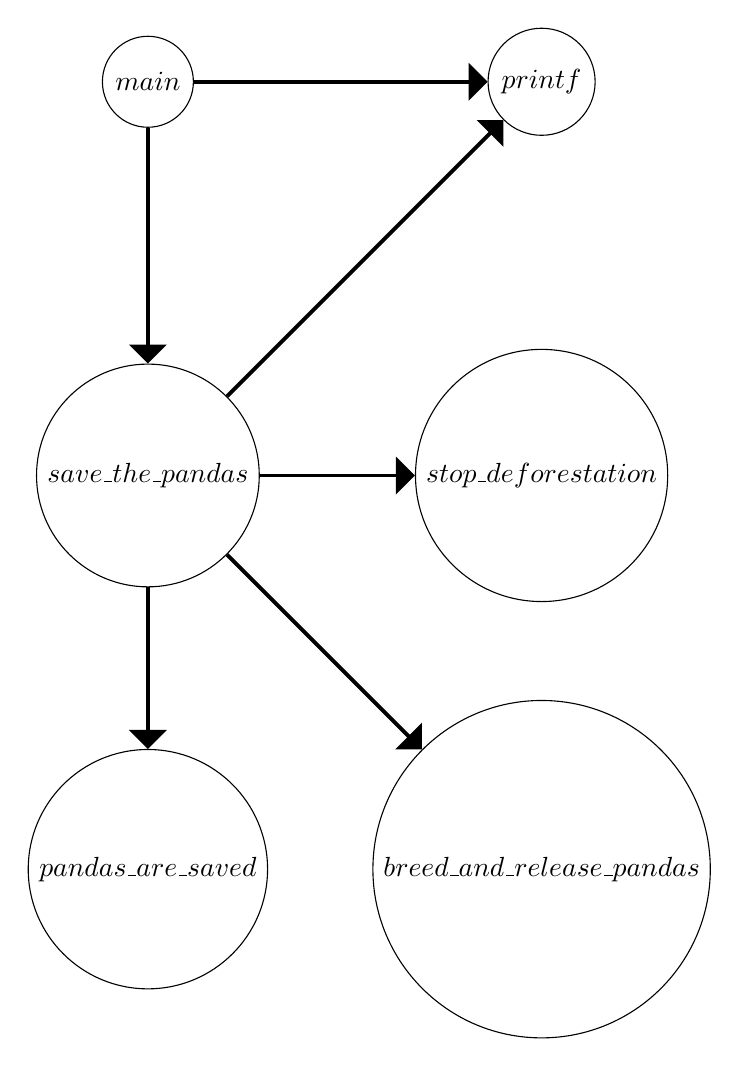
\begin{tikzpicture}[scale=1.0]
        \tikzset{vertex/.style = {shape=circle,draw,minimum size=0.5em}}
        \tikzset{edge/.style = {->,> = latex'}}
        % vertices
        \node[vertex] (main) at  (0,0) {$main$};
        \node[vertex] (savethepandas) at  (0,-5) {$save\_the\_pandas$};
        \node[vertex] (stopdeforestation) at  (5,-5) {$stop\_deforestation$};
        \node[vertex] (breedandreleasepandas) at  (5,-10) {$breed\_and\_release\_pandas$};
        \node[vertex] (printf) at  (5,0) {$printf$};
        \node[vertex] (pandasaresaved) at (0,-10) {$pandas\_are\_saved$};
        %edges
        \draw[edge, -triangle 90, line width=0.5mm] (main) to (savethepandas);
        \draw[edge, -triangle 90, line width=0.5mm] (main) to (printf);
        \draw[edge, -triangle 90, line width=0.5mm] (savethepandas) to (stopdeforestation);
        \draw[edge, -triangle 90, line width=0.5mm] (savethepandas) to (breedandreleasepandas);
        \draw[edge, -triangle 90, line width=0.5mm] (savethepandas) to (pandasaresaved);
        \draw[edge, -triangle 90, line width=0.5mm] (savethepandas) to (printf);
    \end{tikzpicture}
    \caption{Call Graph for the Save the Pandas code listing}
    \label{fig:pandacallgraph}
\end{figure}


As demonstrated by figure \ref{fig:pandacallgraph}, if there is a call from function $X$ to function $Y$ in the source code, there will be an edge pointing from node $X$ to node $Y$ in the associated call graph. 


% references the kitchen-sink of static checking (what else can get checked?)

\chapter{Related work}\label{sec:related}

Static program analysis is a hot topic in Computer Science research.  The Association for Computing Machinery publishes several journals that are focused (at least in part) on static verification and type systems.  It should come as no surprise that there is a large body of research that is related to this thesis.  This Chapter references a tiny fraction of this body of work.  Section \ref{sec:related:effectiveness} calls upon past research to assert unquestionably the positive impact that static analysis has on the software development process.  Section \ref{sec:related:aftermarket} explores a line of research dedicated to inserting supplemental specifications into existing programming languages in order to improve the static checkability of those languages.  Lastly, Section \ref{sec:related:libclang} pays respect to the LLVM project which has enabled so much of this research to happen.

\section{On the Effectiveness of Static Analysis}\label{sec:related:effectiveness}

Studies have long shown that Static Analysis is an essential tool for developing high-quality software.  The high speed and low cost of this type of verification make it an economical method for finding faults in program code \cite{staticanal, static-anal-experience}.  

Industry has taken this observation to heart.  Many companies have their own internal tools dedicated to statically checking code changes with a goal of detecting common mistakes and stylistic issues.  The Mozilla project is a good example of this --- since the early 2000s, Mozilla has used a fairly robust suite of internal tools specifically crafted for Mozillla's mostly C++ codebase.  Using these tools, every Pull Request into Mozilla Firefox is parsed and checked against a set of hand-written rules to detect and report common issues \cite{mozilla-pork-blog, moz-wiki-static-anal}.  Much of this tooling was dedicated to detecting memory issues.  Of course, without modifying the grammar of C++, there are limitations in what can be easily checked statically by these tools.  Only a small subset of the problem could be effectively detected.  

More recently, Mozilla developed and began using a language called Rust which was designed with certain static analysis characteristics in mind.  The Rust language implements an innovative type system meant to formally track the ownership of objects in memory.  ``Rust's type system and runtime guarantee the absence of data races, buffer overflows, stack overflows, and access to uninitialized or deallocated memory'' \cite{rust-is-dope}.  A common sentiment in the Rust-language community is that even though the ``Borrow Checker'' (the part of the type system that enforces memory safety) seems complicated at first, seasoned Rust users learn to depend on it to help them reason through complicated programs  \cite{rust-lang-spec}.  Rust demonstrates that making a type system more expressive and more restrictive can improve both the static checkability of a programming language and also the help the users of those languages.  

\section{Aftermarket Type Systems --- Supplementing an Existing Language}\label{sec:related:aftermarket}

The idea of introducing new forms of type checking into an existing language to increase safety is nothing new.  As early as 1994 tools such as LCLint have existed which allow the programmer to write down specifications about their code that are not necessarily supported by the original language standard.  The LCLint tool can take program source code as well as a file containing supplemental specifications and perform static analysis that is more thorough and informed than could possibly be achieved based on the language standard alone \cite{lclint-og}. 

A useful attribute of these supplemental static analysis tools is that they scale incrementally --- the programmer can use these tools to whatever extent they find helpful and can increase or reduce the amount of information they pass on to these tools as they see fit.  Since these specifications are opt-in, adding new forms of specification to a tool like LCLint is a straightforward way to expand the scope of the tool without breaking backwards compatibility.  As an example, in 1996, Evans \textit{et al}. added a few variable type annotations to LCLint such as \code{not-null}, \code{possibly-null}, and \code{null}.  When used by the programmer, these annotations allow LCLint to check for certain kinds of errors relating to nullness and memory allocation \cite{lclint-memory}.  Such modifications require zero action by the users that choose not to use them; if a variable is not annotated then LCLint will not try to check that variable.  However, as the user adds more annotations, LCLint is able to check more variables.  The amount of feedback LCLint is able to provide scales up and down with the amount of annotations in the code.  

In general, variable annotations like \code{not-null} and \code{possibly-null} are very similar in use to the existing system of type qualifiers in the C family of languages.  A canonical example of a type qualifier would be the C \code{const} qualifier; a variable marked \code{const} may be set once at declaration but never updated again (ignoring unsafe casts).  Type qualifiers and annotations like \code{const} and \code{not-null} have two benefits:  First, they declare the intent behind the code so that other programmers reading the code have a better idea of how it works.  Second, they dictate what the program can and cannot do with an identifier so that the compiler or other static checking tool can detect accidental misuse.  However, their use is entirely optional --- the programmer can choose to treat an identifier as \code{const} or \code{not-null} without actually adding the annotation \cite{theory-of-qual}.

``A Theory of Type Qualifiers'' develops this concept in depth and explores the theoretical and practical concerns involved with using type qualifiers in a language \cite{theory-of-qual}.  One of the most relevant observations to the work in this paper is that every type qualifier introduces a form of subtyping.  For all types $T$ and any qualifier $q$, either $T \leq q T$ or $q T \leq T$ depending on $q$.  Here we notate $T$ qualified by $q$ as $q T$ and we notate $X$ is a subtype of $Y$ as $X \leq Y$.  $X \leq Y$ should be interpreted to mean that $X$ can be safely used whenever $Y$ is expected.  For example $\textrm{int} \leq \textrm{const int}$ because in any statement containing a $\textrm{const int}$, one could safely substitute an $int$ however the reverse is not true.  In the same vein, $\textrm{not-null char*} \leq \textrm{char*}$ because any statement referencing a $\textrm{char*}$ could safely be given a $\textrm{not-null char*}$ instead \cite{theory-of-qual}.  In this paper we will apply this concept to the type qualifiers introduced by funqual in order to argue for the correctness of funqual.  

\section{libClang and the Explosion of C++ Tooling}\label{sec:related:libclang}

C++ is difficult to parse \cite{cpp-sucks, libclang-survey, mozilla-pork, parse-cpp}.  Years of language additions, the need for backwards compatibility, and the existence of a text-based preprocessor means that the language grammar is large and complicated.  As a result, even the simplest static analysis tools require a huge amount of complexity to do basic parsing of source code.  Up until relatively recently, many C++ language tools settled on doing a partial parse of the language using approximations and heuristics \cite{libclang-survey}.  This method can lead to artificial constraints on the language or to incorrect interpretations of the source.  

As a result of the LLVM Compiler Infrastructure Project, we now have an excellent set of tools for working with code.  The Clang compiler is a fully featured compiler from the LLVM project that supports a wealth of C-family language standards including C++17.  The LLVM project also provides libClang which exposes a convenient API to the parser and the AST used by the Clang compiler.  libClang enables developers to create their own tools that build on top of Clang's C++ parser.  This means that developers of static analysis tools only need to focus on maintaining their project's contributions rather than supporting an entire parser/AST toolsuite \cite{libclang-survey}.  Funqual is built using libClang and so the work done in this paper was only possible thanks to the work done by the LLVM Compiler Infrastructure Project.  


% is anything like this?  re-iterate how nothing else does call-tree

\chapter{Type Rules}\label{sec:rules}

Funqual checks a program against a type system.  It is a script that takes in source code as well some user-defined call graph rules, does some computation, and prints one of two things: ``This program is well-typed'', or ``This program is not well typed'' (in practice the later case also comes with an explanation as to why the program is not well-typed).  If a program is well-typed, then it is free from call graph rule violations.  If a program is not well-typed, then it may contain one or more errors.

This chapter contains an overview of the rules implemented by funqual as well as a brief exploration of what needs to happen behind the scenes in order to correctly check these rules.  Section \ref{sec:rules:overview} demonstrates the big picture of what these rules are trying to accomplish.  Section \ref{sec:rules:funptrs} explains how type qualifiers are applied to function pointers and how funqual checks them.  Section \ref{sec:rules:rules} is a detailed explanation of each of the call graph constraints supported by funqual.  Finally, Section \ref{sec:rules:special} explains a few special cases and explains how funqual handles them to create a complete call graph.

Note that this chapter focuses only on the conceptual design of funqual and its type system.  For details on how it is implemented or how to use it, refer to \mbox{Chapter \ref{sec:implementation}}.

\section{Overview}\label{sec:rules:overview}

Before doing a deep dive into the specific rules of funqual, let us look at an example.  Recall the save the pandas example from Section \ref{sec:background}.  It is reproduced in this Section as Figure \ref{lst:rules:pandasource} for convenience.  

\begin{figure}
    \begin{lstlisting}[language=C,gobble=8]
        int breed_and_release_pandas() {
            Panda *baby_panda = malloc(sizeof(Panda));
            release_panda(baby_panda);
        }

        int save_the_pandas() {
            stop_deforestation());
            if (pandas_are_saved()) {
                printf("Stopping deforestation saved the pandas!\n");
                return 1;
            }

            breed_and_release_pandas();
            if (pandas_are_saved()) {
                printf("Breeding pandas in captivation and releasing them has saved the pandas!\n");
                return 1;
            }
            return 0;
        }

        int main(void) {
            if (save_the_pandas()) {
                printf("The pandas have been saved!\n");
            }
        }
    \end{lstlisting}
    \caption{Example C program.  Running this code in a production environment may not actually save the pandas}
    \label{lst:rules:pandasource}
\end{figure}

Let us now imagine that there is some constraint whereby \lstinline{save_the_pandas} should not allocate memory. As programmers we would like to believe that we are disciplined enough to remember this rule and enforce it ourselves. In practice, self-regulation like this often ends poorly. As a result we would like a tool like funqual to enforce this constraint automatically.

\begin{sloppypar}
Funqual allows us as programmers to create our own type qualifiers and to apply whatever meaning we want to those qualifiers.  In this particular case we create two type qualifiers: \lstinline{static_memory} and \mbox{\lstinline{dynamic_memory}.} We also create one rule: $restrict\_indirect\_call(static\_memory, dynamic\_memory)$. When the programmer qualifies a function with \lstinline{static_memory}, that declares the intent that this function will \textit{never} allocate memory on the heap. When the programmer qualifies a function with \lstinline{dynamic_memory}, that declares the intent that this function always allocates memory on the heap\footnote{The meanings of these type qualifiers are as determined by the programmer; without a rule to operate on them, funqual will completely ignore the type qualifiers.}. The rule $restrict\_indirect\_call(static\_memory, dynamic\_memory)$ tells funqual that \lstinline{static_memory} functions are not allowed to call \lstinline{dynamic_memory} functions either directly or indirectly. If it is possible for a \lstinline{static_memory} function to reach a \lstinline{dynamic_memory} function, then the rule has been violated and funqual should inform the user.
\end{sloppypar}

In the example about saving the pandas, we would qualify \lstinline{save_the_pandas} as \lstinline{static_memory} and we would qualify \lstinline{malloc} as \lstinline{dynamic_memory}.  Figure \ref{fig:coloredpandacallgraph} shows the call graph for Figure \ref{lst:rules:pandasource} with \lstinline{static_memory} functions marked green and with \lstinline{dynamic_memory} functions marked red.

\input{figures/colored-panda-call-graph}

\begin{sloppypar}
By turning the program into a directed graph and by assigning types to the vertices, we have transformed the problem of type qualifier rule satisfaction into a graph problem.  A question like \textit{are there any static\_memory functions that inadvertently call dynamic\_memory functions} essentially boils down to \textit{are there any paths from green vertices to red vertices}.  In this example, the answer to that question is yes.  In the code, \lstinline{save_the_pandas} calls \lstinline{breed_and_release_pandas} which calls \lstinline{malloc} constituting an illicit call.  Equivalently, \lstinline{save_the_pandas} has an edge to \lstinline{breed_and_release_pandas} which has an edge to \lstinline{malloc} constituting an illicit path.  A well-typed program has no paths from green vertices to red vertices.  A poorly-typed program will have at least one path.  
\end{sloppypar}




\section{Function Pointers and Indirect Type}\label{sec:rules:funptrs}

Traversing a program for function calls and adding them to the call graph is relatively straightforward.  Knowing exactly what function is being called at the time of parsing makes this process trivial.  This does not account for all function calls, however.  There are multiple cases in modern C++ where a function call is either happening behind the scenes or where the exact callee is not knowable.  This section examines function pointers and explains how they are represented in the call graph.  

As a concrete example, refer to Listing \ref{lst:rules:ptreg}.  In this example, it is literally impossible to know what function \lstinline{strat} is going to point to.  This is a pointed example, but \lstinline{rand} can represent any expression whose result is unknowable during static analysis.  Additionally, in this example there are very clearly only three functions that \lstinline{strat} could point to.  In a real program, there might be thousands of functions and they might not all be listed in one place.  

\noindent\begin{minipage}[t]{\linewidth}
\begin{lstlisting}[language=C,caption={In this example C program, it is impossible to know statically what the value of \lstinline{strat} is.  Because of this, funqual requires the programmer to annotate function pointers with additional type information. },label={lst:rules:ptreg}]
int breed_and_release_pandas() {
    Panda *baby_panda = malloc(sizeof(Panda));
    return release_panda(baby_panda);
}

int (*)() get_random_strategy() {
    switch (rand() % 3) {
        case 0:
            return breed_and_release_pandas;
            break;
        case 1:
            return stop_deforestation;
            break;
        case 2:
            return stop_hunting;
            break;
    }
}

int save_the_pandas() {
    while (!pandas_are_saved()) {
        int (*strat)() = get_random_strategy()
        strat();
    }
    return 0;
}

int main(void) {
    return save_the_pandas();
}
\end{lstlisting}
\end{minipage}

\begin{sloppypar}
If we still intend to use funqual to enforce this $restrict\_indirect\_call(\allowbreak static\_memory, dynamic\_memory)$ rule then we are going to need some additional tools.  Since keeping track of all the possile values of \lstinline{strat} is impractical, we will instead keep track of the type of \lstinline{strat} with respect to this call graph.  Recall that the type of \lstinline{save_the_pandas} is \lstinline{static_memory} and that the type of \lstinline{malloc} is \lstinline{dynamic_memory}.  If we had a function pointer pointing to \lstinline{malloc}, then the type of that function pointer would have to also be \lstinline{dynamic_memory}.  In this example we have a function pointer pointing to \lstinline{breed_and_release_pandas}.  We will say that \lstinline{breed_and_release_pandas} has \textit{indirect type} \lstinline{dynamic_memory} because it calls \lstline{malloc} and so any function pointer that points to \lstinline{breed_and_release_pandas} must have indirect type \lstinline{dynamic_memory}.
\end{sloppypar}

For this reason, when we use function pointers we will have two kinds of type qualifiers:  \textit{direct type} qualifiers and \textit{indirect type} qualifiers.  Direct type refers to the funqual type qualifiers we have explicitly assigned to the pointee.  Indirect type refers to the funqual type qualifiers of all the functions reachable from the pointee.  Direct type for both functions and function pointers must be explicitly annotated in the code.  Indirect types for function pointers must be annotated explicitly but can be inferred automatically for functions. 

Listing \ref{lst:rules:pandaptrannote} shows the same code as Listing \ref{lst:rules:ptreg} but with function types annotated.  Figure \ref{fig:rules:pandaptrannote} shows the call graph for Listing \ref{lst:rules:pandaptrannote} with the function pointer represented as a cloud.  Notice that we do not need to write any explicit annotations for the indirect type of \lstinline{breed_and_release_pandas}.  Funqual has all the information it needs to statically infer the indirect type of functions.  In this case, the indirect type is \lstinline{dynamic_memory} because \lstinline{breed_and_release_pandas} calls \lstinline{malloc}.  Also notice that \lstinline{strat} has indirect type \lstinline{dynamic_memory}.  This matters because it is \textit{possible} that calling \lstinline{strat} might result in a \lstinline{dynamic_memory} function getting called.  

\noindent\begin{minipage}[t]{\linewidth}
\begin{lstlisting}[language=C,caption={Same example program as Listing \ref{lst:rules:ptreg} but with function pointer type annotations inserted},label={lst:rules:pandaptrannote}]
int breed_and_release_pandas() {
    Panda *baby_panda = malloc(sizeof(Panda));
    return release_panda(baby_panda);
}

int indirect_dynamic_memory (*)() get_random_strategy() {
    switch (rand() % 3) {
        case 0:
            return breed_and_release_pandas;
            break;
        case 1:
            return stop_deforestation;
            break;
        case 2:
            return stop_hunting;
            break;
    }
}

int save_the_pandas() static_memory {
    while (!pandas_are_saved()) {
        int indirect_dynamic_memory (*strat)() =
            get_random_strategy()
        strat();
    }
    return 0;
}

int main(void) {
    return save_the_pandas();
}
\end{lstlisting}
\end{minipage}

\begin{figure}
    \centering
    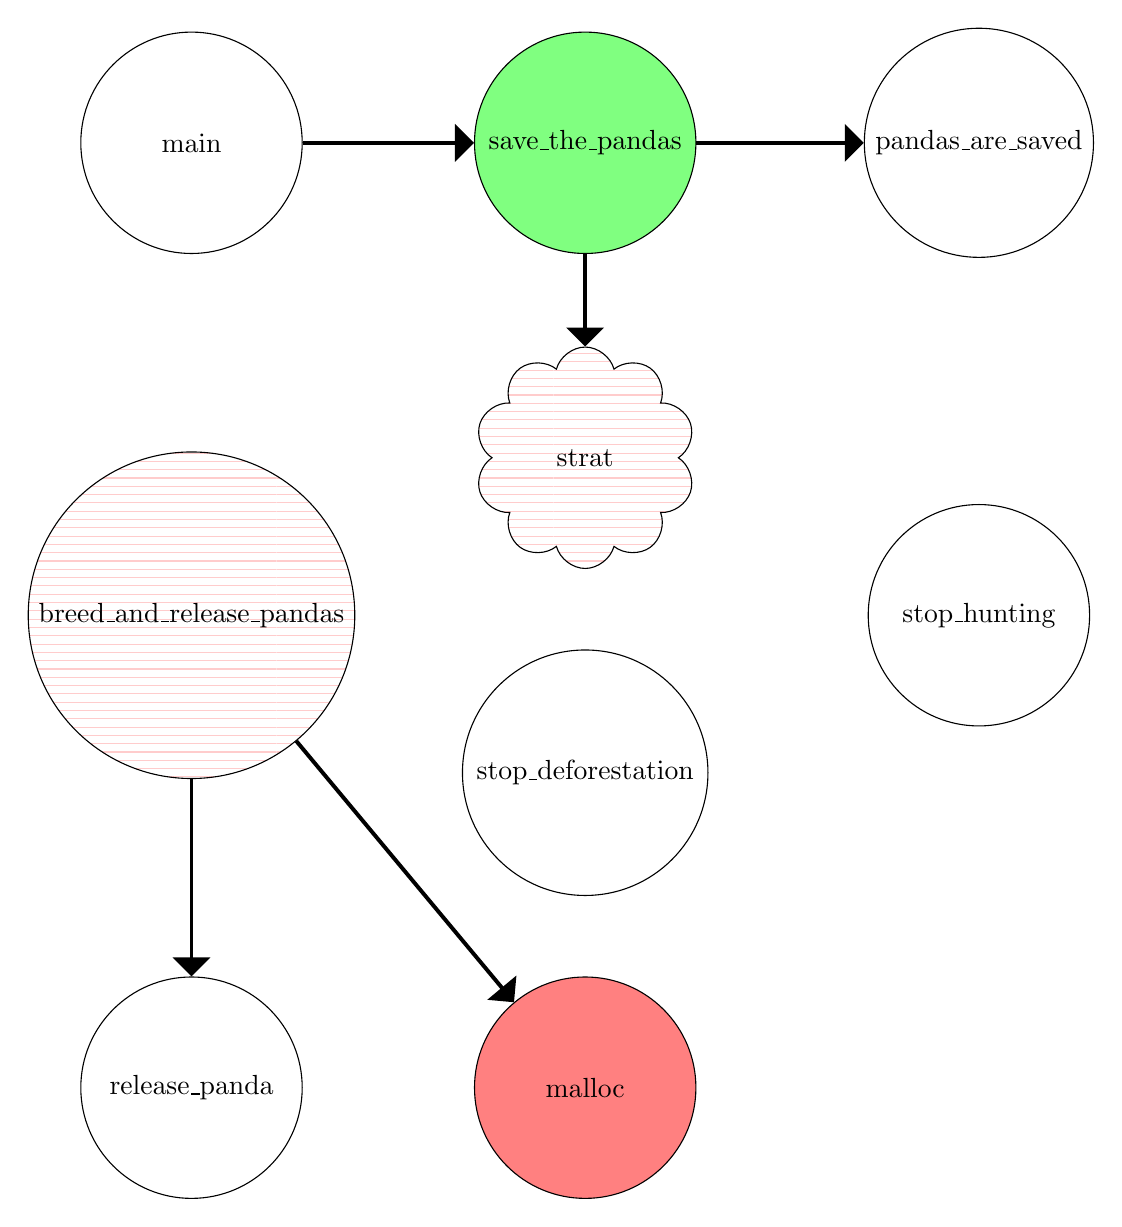
\begin{tikzpicture}[scale=1.0]
        \tikzset{vertex/.style = {shape=circle,draw,minimum size=8em}}
        \tikzset{edge/.style = {->,> = latex'}}
        % vertices
        \node[vertex] (main) at  (0, 0) {\lstinline{main}};
        \node[vertex, fill=green!50]
            (savethepandas) at  (5, 0) {\lstinline{save_the_pandas}};
        \node[vertex] (pandasaresaved) at (10, 0) {\lstinline{pandas_are_saved}};
        \node[vertex, shape=cloud, pattern=horizontal lines, pattern color=red!20]
            (strat) at (5, -4) {\lstinline{strat}};
        \node[vertex] (stopdeforestation) at  (5, -8) {\lstinline{stop_deforestation}};
        \node[vertex] (stophunting) at (10, -6) {\lstinline{stop_hunting}};
        \node[vertex, pattern=horizontal lines, pattern color=red!20]
            (breedandreleasepandas) at (0, -6)
            {\lstinline{breed_and_release_pandas}};
        \node[vertex] (releasepanda) at (0, -12) {\lstinline{release_panda}};
        \node[vertex, fill=red!50] (malloc) at (5, -12) {\lstinline{malloc}};
        %edges
        \draw[edge, -triangle 90, line width=0.5mm] (main) to (savethepandas);
        \draw[edge, -triangle 90, line width=0.5mm] (savethepandas) to (strat);
        \draw[edge, -triangle 90, line width=0.5mm] (savethepandas) to (pandasaresaved);
        \draw[edge, -triangle 90, line width=0.5mm] (breedandreleasepandas) to (releasepanda);
        \draw[edge, -triangle 90, line width=0.5mm] (breedandreleasepandas) to (malloc);
    \end{tikzpicture}
    \caption{Color-coded Call Graph for Listing \ref{lst:rules:pandaptrannote}.  Functions tagged \lstinline{static_memory} are highlighted green and functions tagged \lstinline{dynamic_memory} are highlighted red.  Indirect types are represented as horizontal line patterns on a node.  Clouds represent function pointers.}
    \label{fig:rules:pandaptrannote}
\end{figure}

Thanks to the graph based representation of this program, it is clear to see where the error is.  \lstinline{save_the_pandas} calls \lstinline{strat} and it is possible that a call to \lstinline{strat} could result in a call to \lstinline{malloc}.  The indirect type of \lstinline{strat} (notated in Figure \ref{fig:rules:pandaptrannote} as red horizontal lines) is how we keep track of this possibility.  

%\subsection{Indirect Type Inference}
%
%As mentioned earlier, funqual is able to infer the indirect type of functions.  For any function, $F$, the indirect type can be determined by traversing the call graph and visiting all the vertices that are reachable from $F$.  The indirect type of $F$ is the union of the direct types and indirect types of all the vertices that $F$ can reach.  
%
%Once again, the indirect type of $F$ is a list of types that could \textit{possibly} be reached from a call to $F$.  If we are trying to enforce a $restrict\_indirect\_call(X, Y)$ rule, it is important that under no circumstance, following no execution path, is it possible for a function in $X$ to call a function in $Y$.  Taking this expansive view of indirect type is the only way to guarantee call graph safety.  
%
%This indirect type inference is only possible because the body of the function can be found and traversed statically.  For function pointers, there is no way of knowing which functions the pointer can reference.  As a result, indirect type for function pointers must be annotated explicitly and every assignment into the function pointer is checked to ensure that the assignment does not lose any type information.

\subsection{Rules of Assignment}

To properly enforce call graph constraints, funqual checks function pointers in two places:  first when the function pointer is assigned, and second when the function pointer is called.  The rules described in this section are crafted specifically to maintain call graph correctness.  For the purpose of this discussion, we will let $L$ stand for some function pointer and we will let $R$ stand for some function value (the names $L$ and $R$ are a reference to the \lstinline{lvalue} and \lstinline{rvalue} in a typical assignment statement).  

When assigning a function pointer $L$ to point to a function $R$, there are two rules that funqual checks:  The direct type of $L$ must match exactly the direct type of $R$, and the indirect type of $L$ must be the superset of the indirect type of $R$.  For function pointers, both the direct and indirect types must be explicitly annotated in code.  For functions, only the direct type must be explicitly annotated as the indirect type can be inferred.  

These rules are necessary to maintain the soundness of the system.  In order to correctly enforce $require\_direct\_call(X, Y)$, the direct type of $L$ must be contained in $R$ --- otherwise a call to $L$ might be considered valid even if $R$ does not have $Y$ in its type.  In order to correctly enforce $restrict\_direct\_call(X, Y)$, the direct type of $R$ must be contained in $L$ --- otherwise a call to $L$ might be considered valid even if $R$ does not have $Y$ in its type.  Combining both of these requirements means that the direct types of $L$ and $R$ must match exactly.  Lastly, in order to properly enforce $restrict\_indirect\_call(X, Y)$, we need to know all the funqual types that are possibly reachable by calling $L$.  

Table \ref{fig:rules:assignment_table} shows a few examples of valid and invalid assignments.  

\begin{table}
    \centering
    \begin{tabular}{|c|c|c|c|c|}
        \hline
        lvalue & lvalue & rvalue & rvalue & Valid? \\
        direct & indirect & direct & indirect & \\
        \hline
        \hline
        \rowcolor{tablegreen}
        (none) & (none) & (none) & (none) & Valid \\
        \hline
        \rowcolor{tablered}
        static\_memory & (none) & (none) & (none) & Not Valid \\
        \hline
        \rowcolor{tablered}
        (none) & (none) & static\_memory & (none) & Not Valid \\
        \hline
        \rowcolor{tablegreen}
        static\_memory & (none) & static\_memory & (none) & Valid \\
        \hline
        \rowcolor{tablegreen}
        static\_memory & blocking & static\_memory & (none) & Valid \\
        \hline
        \rowcolor{tablered}
        static\_memory & (none) & static\_memory & blocking & Not Valid \\
        \hline
        \rowcolor{tablegreen}
        static\_memory & blocking & static\_memory & blocking & Valid \\
        \hline
        \rowcolor{tablered}
        static\_memory & blocking & static\_memory & nonblocking & Not Valid \\
        \hline
        \rowcolor{tablegreen}
        static\_memory & blocking & static\_memory & nonblocking & Valid \\
        \rowcolor{tablegreen}
         & nonblocking &  & & \\
        \hline
        \rowcolor{tablegreen}
        (none) & blocking & (none) & (none) & Valid \\
        \rowcolor{tablegreen}
         & static\_memory & & & \\ 
        \rowcolor{tablegreen}
         & nonblocking & & & \\ 
        \hline
    \end{tabular}
    \caption{Examples of valid and invalid assignments in funqual.  The left two collumns show the direct and indirect type of the lvalue respectively.  The next two columns show the direct and indirect type of the rvalue respectively.  The rightmost column shows whether or not that assignment is valid.}
    \label{fig:rules:assignment_table}
\end{table}




\section{Call Graph Rules}\label{sec:rules:rules}

% X and Y are type qualifiers (sets of functions)
% E is set of edges
% P is set of paths
% A and B are functions

Each subsection here describes one of the call graph rules supported by funqual.  For each rule, we explain the meaning, provide an algorithm that could enforce it, and present an argument for the algorithm's correctness with respect to the rest of the type system.  The algorithms presented here only return \lstinline{true} or \lstinline{false} depending on whether the graph in question is valid.  The algorithms actually implemented in funqual are slightly more complicated because they print helpful diagnostic messages to the user.  Both sets of algorithms enforce the same rules, though.  

\subsection{Restrict Direct Call}

\begin{center}
    $restrict\_direct\_call(X, Y)$
\end{center}

A restrict direct call rule creates a constraint that disallows functions with direct type $X$ from calling functions with direct type $Y$.  This constraint is relatively permissive because it still allows indirect calls from functions with direct type $X$ to functions with direct type $Y$ but is nonetheless checkable by this type system.

Figure \ref{lst:rules:rules:restrict_direct_call} shows pseudocode for an algorithm that can check a call graph for violations of this rule.  Assume that \lstinline{edges} is a list of objects representing all the calls in the call graph.  

\begin{figure}
    \begin{lstlisting}[gobble=8]
        function enforce_restrict_direct_call(X, Y, edges):
            for edge in edges:
                callee = edge.to
                caller = edge.from

                if X in caller.direct_type and Y in callee.direct_type:
                    return false
            return true
    \end{lstlisting}
    \caption{Pseudocode for an algorithm that can check a $restrict\_direct\_call$ constraint.  This algorithm returns \lstinline{true} if the call graph respects the constraint and \lstinline{false} if the call graph violates it.}
    \label{lst:rules:rules:restrict_direct_call}
\end{figure}

This algorithm runs once per rule and terminates in linear time with respect to the number of edges in the call graph.  To assert the correctness of this algorithm we will categorize each function call in this graph as one of two possibilities:  a call to a standard function, or a call to a function pointer.

\interfootnotelinepenalty=10000

In the case of a standard function call, the correctness is trivial.  The user must have annotated the direct type of both the caller and the callee\footnote{Funqual will check whatever was declared by the programmer --- whether the programmer declared their intent correctly is outside the scope of this research.}.  If a function with direct type $X$ calls a function with direct type $Y$, then \lstinline{edges} will contain such an edge and in checking each edge we will detect it.  

In the case of the function pointer call, we need to also examine all possible assignments of that function pointer.  It is of course possible that the function pointer is null at runtime, but we will consider this type of error to be out of the scope of funqual.  For the sake of this argument, let $P$ stand for any function pointer and $F$ stand for any function.  For an assignment of $F$ into $P$ to be valid, $F$ and $P$ must have the same direct type.  If they do not have the same direct type, then funqual will inform the user of an assignment type violation.  If they do have the same direct type, then \lstinline{edges} will contain an edge into $P$ wherever $P$ is called and that edge will be checked in the same way as a standard function call.  

\subsection{Restrict Indirect Call}

\begin{center}
    $restrict\_indirect\_call(X, Y)$
\end{center}

A restrict indirect call rule creates a constraint that functions with direct type $X$ cannot call functions with direct or indirect type $Y$.  This has the effect of restricting functions with direct type $X$ from calling functions with direct type $Y$, whether that call is direct or indirect.  The need to enforce indirect calls in the presence of function pointers requires us to examine the indirect type of the callee for each edge.  

\begin{figure}
    \begin{lstlisting}[gobble=8]
        function enforce_restrict_indirect_call(X, Y, edges):
            for edge in edges:
                callee = edge.to
                caller = edge.from

                if X in caller.direct_type and Y in callee.indirect_type:
                    return false
            return true
    \end{lstlisting}
    \caption{Pseudocode for an algorithm that can check a $restrict\_indirect\_call$ constraint.  This algorithm returns \lstinline{true} if the call graph respects the constraint and \lstinline{false} if the call graph violates it.}
    \label{lst:rules:rules:restrict_indirect_call}
\end{figure}

Figure \ref{lst:rules:rules:restrict_indirect_call} shows pseudocode for an algorithm that can check a call graph for violations of this rule.  Assume that \lstinline{edges} is a list of objects representing all the calls in the call graph.  

In order to simplify this algorithm, we will assume for the time being that indirect function types are inferred correctly.  For an explanation of the indirect type inference algorithm and for an argument for its correctness, refer to Subsection \ref{sec:rules:rules:inference}.  To assert the correctness of \lstinline{enforce_restrict_indirect_call}, we will again consider each function call in the graph as a member of one of two categories: a call to a standard function, or an invocation of a function pointer.

In the case of a standard function call, the correctness is trivial.  Assume function $A$ with direct type $X$ calls function $B$ with indirect type $Y$.  Since $A$ directly calls $B$, we know that there will be an edge from $A$ to $B$ in the \lstinline{edges} and when the algorithm visits it, the algorithm will terminate with the claim that there is a violation.

In the case of a function pointer invocation, the rules of function pointer assignment come into play.  If, via an invocation of $B$, a function of type $Y$ could eventually be called, then the function pointer must necessarily have $Y$ in its indirect type otherwise there would be an assignment error (for an in-depth argument of this refer to Subsection \ref{sec:rules:rules:inference}).  As a result, when visiting the edge from $A$ to $B$ (where $A$ is the function invoking function pointer $B$), the algorithm will detect that $B$ has indirect type $Y$ and will terminate with the claim that there is a violation.  

\subsection{Require Direct Call}

\begin{center}
    $require\_direct\_call(X, Y)$
\end{center}

A require direct call rule creates a constraint that functions with direct type $X$ can only call functions with direct type $Y$. Much like the restrict direct call rule, this rule is relatively easy to check and can be checked in time linear with respect to the number of edges in the call graph.

Figure \ref{lst:rules:rules:require_direct_call} shows pseudocode for an algorithm that can check a call graph for violations of this rule.  Assume that \lstinline{edges} is a list of objects representing all the calls in the call graph.  

\begin{figure}
    \begin{lstlisting}[gobble=8]
        function enforce_require_direct_call(X, Y, edges):
            for edge in edges:
                callee = edge.to
                caller = edge.from

                if X in caller.direct_type and Y not in callee.direct_type:
                    return false
            return true
    \end{lstlisting}
    \caption{Pseudocode for an algorithm that can check a $require\_direct\_call$ constraint.  This algorithm returns \lstinline{true} if the call graph respects the constraint and \lstinline{false} if the call graph violates it.}
    \label{lst:rules:rules:require_direct_call}
\end{figure}

To assert the correctness of this algorithm, we will categorize every function call as one of two possibilities: a call to a standard function, or a call to a function pointer.

In the case of a call to a standard function, the correctness is trivial.  The user must have annotated the direct type of both the caller and the callee and we take these annotations to be correct.  If a function with direct type $X$ calls any function, then \lstinline{edges} will contain an edge from the caller to the callee.  Checking the direct types of caller and callee exhaustively for every edge in the graph will eventually find any violations.

In the case of a function pointer call, we need to also examine all the possible assignments to that function pointer.  Thankfully the assignment checker already checked the type safety of every function pointer assignment so we will assume that those are correct.  In this case specifically, we can assume that, if the function which is actually called does not have direct type $Y$, then the function pointer which is called in code will also not have direct type $Y$.  This call creates an edge which will certainly be visited by \lstinline{enforce_restrict_direct_call} and so we can be certain that any function pointer invocation will be correctly checked in this regard.

\subsection{Indirect Type Inference}\label{sec:rules:rules:inference}

While the user does not invoke indirect type inference in the same way that the user invokes the other rules, indirect type inference is still an important part of the type safety of funqual.  This subsection explains indirect type inference and argues for the correctness of the algorithm.  

Figure \ref{lst:rules:rules:infer_indirect_type} shows pseudocode for an algorithm that can infer the indirect function type for any function in the call graph.  For the purpose of this function, we will let \lstinline{function} be the function being checked.  We will let \lstinline{edges} be the list of edges in our graph and we will assume that it contains edges to function pointers where those function pointers are called.  We also assume that \lstinline{callee.indirect_type} is populated for function pointers but that it is an empty set for regular functions.  

\begin{figure}
    \begin{lstlisting}[gobble=8]
        function infer_indirect_type(function, edges):
            indirect_types = empty set
            visited = empty set
            to_visit = empty set
            to_visit.add(function)

            while to_visit is not empty:
                curr = to_visit.pop()
                visited.add(curr)

                indirect_types.add_all(curr.direct_type)
                indirect_types.add_all(curr.indirect_type)

                for edge in edges:
                    callee = edge.to
                    caller = edge.from
                    if caller == curr and callee not in visited:
                        to_visit.add(callee)
            return indirect_types
    \end{lstlisting}
    \caption{Pseudocode for an algorithm to infer the indirect type of a function.}
    \label{lst:rules:rules:infer_indirect_type}
\end{figure}

To assert the correctness of this algorithm imagine a function, $F$, from which evaluation eventually (either directly or indirectly) reaches a function, $C$, with type $Y$.  We propose that because of the rules of this type system, it is necessary that $Y$ is in the type of $F$.  To demonstrate this we will break down the type pipeline into its multiple cases.

The first case is that $F$ calls $C$ (either directly or indirectly) but that none of the calls from $F$ to $C$ are function pointer invocations.  In this case, there will be a path in \lstinline{edges} from $F$ to $C$ and because \lstinline{infer_indirect_type} is a breadth first graph traversal starting at $F$, we know that the algorithm will eventually visit $C$.  When the algorithm does visit $C$, it will grab the direct type of $C$ (which contains $Y$) and add it to the indirect type of $F$.  When the algorithm terminates, it will necessarily contain $Y$.  In other words, if there is a path from $F$ to $C$, the indirect type of $F$ will contain the direct and indirect types of $C$.

The second case is that $F$ invokes a function pointer $P$ from which evaluation eventually results in a call to $C$.  In this case, there may or may not be a path in \lstinline{edges} from $F$ to $C$.  However, there will be a path in \lstinline{edges} from $F$ to $P$ and an assignment of $C$ into $P$.  Recall that for an assignment of $C$ into $P$ to typecheck, the direct types of $C$ and $P$ must match and the indirect type of $P$ must contain the indirect type of $C$.  If $Y$ is in the direct type of $C$, then $Y$ must be in the direct type of $P$.  Also if $Y$ is in the indirect type of $C$, then $Y$ must be in the indirect type of $P$.  Since either the direct type or the indirect type of $P$ must contain $Y$, we can reference case one and claim that because there is a path from $F$ to $P$, and because the type of $P$ contains $Y$, then $Y$ will be in the indirect type of $F$.  

The third case is an inductive step.  Assume that $F$ calls $C$ but indirectly through some arbitrary number of function pointer invocations between.  Let $P_0$ be a function pointer through which a call is made to $C$, let $P_1$ be a function pointer through which a call is made to $P_0$, let $P_n$ be a function pointer through which a call is made to $P_{n-1}$, and let $F$ call $P_n$.  According to the logic in case two, if $Y$ is in the direct type of $C$, then it must be in the direct type of $P_0$ or else the assignment will have failed.  In the same way, if $Y$ is in the direct or indirect type of $P_{n-1}$, then it must be in the direct or indirect type of $P_{n}$.  Inductively, $Y$ must be in the direct or indirect type of $P_n$ and because there is a path in \lstinline{edges} from $F$ to $P_n$, $Y$ must end up in the indirect type of $F$.  Lastly, as in case one, any of these calls (either from $F$ to $P_n$, from $P_n$ to $P_{n-1}$, or from $P_0$ to $C$) can be direct or indirect calls and $Y$ will still be in the indirect type of $F$.

This algorithm terminates even in the presence of cycles because it tracks previously visited vertices in \lstinline{visited} and does not visit them again.  Even though these cyclic edges are not followed, the output is still correct because every vertex is visited once.  Assume that $F$ calls $C$ and that $C$ calls $F$.  The algorithm first visits $F$, then visits $C$, but does not visit $F$ again because $F$ was added to \lstinline{visited} when it was first examined.  When $F$ was added to \lstinline{visited}, its direct and indirect type were added to the return value and the edges out of $F$ were added to \lstinline{to_visit}.  All the necessary information was extracted from $F$ on the first visit so visiting it again is not necessary.


\section{Special Considerations when Creating a Call Graph}\label{sec:rules:special}

\subsection{Dealing with Inheritance}\label{sec:rules:inherit}

When calling a virtual method in C++, it is impossible to know at compile time exactly which function is going to be run at run-time.  This is very similar to the problem of function pointers (and in fact dynamic dispatch is usually implemented as a table of function pointers \cite{language-standard}) except that in the case of virtual functions we actually know statically the set of possible functions that could be called\footnote{Funqual assumes that it has access to the full source code for call graph creation.}.  To account for this, we need to add extra edges to our call graph to represent all the possible places that a virtual method call could go.  

Let $C$ be some function that calls $T.M$ where $T$ is some class and $M$ is a virtual method of $T$.  When creating the call graph, we must surely add an edge from $C$ to $T.M$.  In addition to that, though, for any class $S$ that is a subclass of $T$, we must also add an edge from $C$ to $S.M$.  This accounts for any possible overloads of $M$ that might be called at run-time.

Figure \ref{lst:rules:inheritance} demonstrates this concept.  It is a piece of C++ source code that calls a virtual function.  Figure \ref{fig:rules:inheritance} shows the call graph for this code sample.  

\begin{figure}
    \begin{lstlisting}[language=C++,gobble=8]
        class Panda {
        protected:
            int m_hunger;
        public:
            virtual int Feed() {
                m_hunger--;
            }
        };

        class RedPanda : public Panda{
        public:
            int Feed() override {
                Stomach *stomach = malloc(sizeof(Stomach));
                memset(stomach, 0xFF, sizeof(Stomach));
            }
        };

        void feedPanda(Panda *panda) static_memory {
            panda->Feed();
        }

        int main(void) {
            feedPanda(new RedPanda());
        }
    \end{lstlisting}
    \caption{Example C++ program demonstrating inheritance.  In \lstinline{feedPanda}, it is impossible to know statically which instance of the \lstinline{Feed} function will be called.  Figure \ref{fig:rules:inheritance} shows the call graph for this program.}
    \label{lst:rules:inheritance}
\end{figure}

\begin{figure}
    \centering
    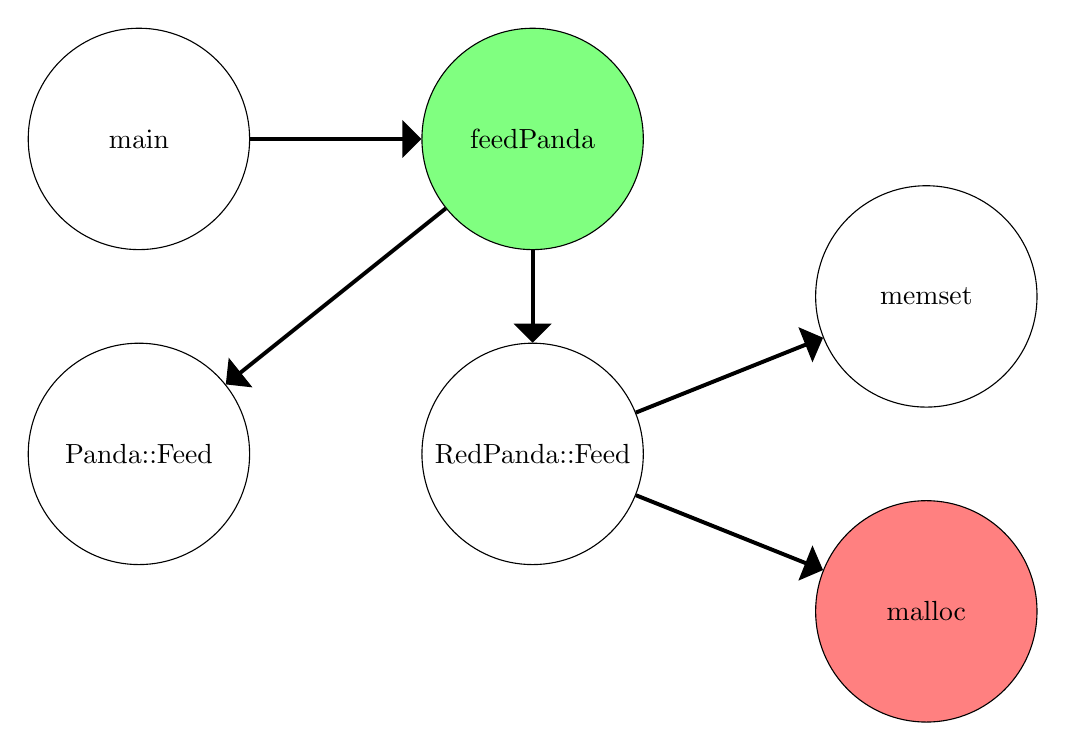
\begin{tikzpicture}[scale=1.0]
        \tikzset{vertex/.style = {shape=circle,draw,minimum size=8em}}
        \tikzset{edge/.style = {->,> = latex'}}
        % vertices
        \node[vertex] (main) at  (0, 0) {\lstinline{main}};
        \node[vertex, fill=green!50] (feedPanda) at  (5, 0) {\lstinline{feedPanda}};
        \node[vertex] (PandaFeed) at (0, -4) {\lstinline{Panda::Feed}};
        \node[vertex] (RedPandaFeed) at  (5, -4) {\lstinline{RedPanda::Feed}};
        \node[vertex] (memset) at  (10, -2) {\lstinline{memset}};
        \node[vertex, fill=red!50] (malloc) at  (10, -6) {\lstinline{malloc}};
        %edges
        \draw[edge, -triangle 90, line width=0.5mm] (main) to (feedPanda);
        \draw[edge, -triangle 90, line width=0.5mm] (feedPanda) to (PandaFeed);
        \draw[edge, -triangle 90, line width=0.5mm] (feedPanda) to (RedPandaFeed);
        \draw[edge, -triangle 90, line width=0.5mm] (RedPandaFeed) to (malloc);
        \draw[edge, -triangle 90, line width=0.5mm] (RedPandaFeed) to (memset);
    \end{tikzpicture}
    \caption{Call graph for Figure \ref{lst:rules:inheritance}.  Because \lstinline{Panda::Feed} is a virtual function, we must draw an edge from \lstinline{feedPanda} to every instance of \lstinline{Feed}.}
    \label{fig:rules:inheritance}
\end{figure}

For this example we will continue to assume that there is a rule restricting indirect calls from \lstinline{static_memory} functions to \lstinline{dynamic_memory} functions.  In \lstinline{feedPanda} we can see that we call \lstinline{Panda::Feed}.  This is somewhat misleading:  \lstinline{Panda::Feed} is a virtual function and it is overridden by a child class called \lstinline{RedPanda}.  This means that any time \lstinline{feedPanda} is called, it is impossible to know whether it is \lstinline{Panda::Feed} being called or whether it is actually \lstinline{RedPanda::Feed} being called.  The only safe way to handle this scenario is to assume that \lstinline{feedPanda} calls both of them.  This is reflected in Figure \ref{fig:rules:inheritance} which is a call graph showing \lstinline{feedPanda} pointing to both versions of the \lstinline{Feed} function.  

\subsection{Overriding Methods with Annotations}

Just like with the standard C++17 type qualifiers, if a virtual function $T.M$ is overridden by $S.M$, then the qualified types of $T.M$ and $S.M$ must match exactly.  Figure~\ref{lst:rules:bad_override} contains an example of an override that is invalid according to the C++17 standard.  In this example, \lstinline{Panda::Feed} has a \lstinline{const} qualifier, but \lstinline{RedPanda::Feed} does not.  As such, the two functions have different types and the compiler will generate an error.  

\begin{figure}
    \begin{lstlisting}[language=C++,gobble=8]
        class Panda {
        public:
            virtual void Feed() const;
        };

        class RedPanda: public Panda {
            virtual void Feed() override;
        };
    \end{lstlisting}
    \caption{Example C++ containing an error.  \lstinline{Panda::Feed} and \lstinline{RedPanda::Feed} have different types and so the override is invalid.}
    \label{lst:rules:bad_override}
\end{figure}

Funqual treats funqual direct type in the same way.  For $T.M$ to be overridden by $S.M$, the two functions must have the same direct type.  If they do not, funqual will display an error.  The Figure~\ref{lst:rules:bad_override_qtag} shows a similar example of an invalid override but where the direct type is the type in conflict.

\begin{figure}
    \begin{lstlisting}[language=C++,gobble=8]
        class Panda {
        public:
            virtual void Feed() QTAG(static_memory);
        };

        class RedPanda: public Panda {
            virtual void Feed() override;
        };
    \end{lstlisting}
    \caption{Example C++ containing a funqual type error.  \lstinline{Panda::Feed} and \lstinline{RedPanda::Feed} have different types and so the override is invalid.}
    \label{lst:rules:bad_override_qtag}
\end{figure}

\subsection{Operator Overloading}

C++ allows for operator overloading.  As a result, an expression such as \mbox{\lstinline{a = b + c;}} could result in a function call depending on the types of \lstinline{a} and \lstinline{b}.  

Compensating for this is relatively straightforward.  When funqual comes across a binary or unary operator that can be overloaded, it checks the type of the operand(s) and checks for an operator overload.  If there is an operator overload, then the call graph will contain an edge from the calling context to the overload function.  If the overload is virtual, funqual checks for operator overloads in child classes as described in Section \ref{sec:rules:inherit}.

\subsection{Bridging the Divide between Translation Units}

The compilation of C++ code is driven by translation units.  Translation units are the files which are provided to the C compiler to be translated into object files.  In general, translation units are singular \lstinline{.c} or \lstinline{.cpp} files including any source files that may be \lstinline{#include}-ed.  During this process, many symbols are said to have \textit{external linkage} meaning that their type is specified in this translation unit but that their value is not (this is the case with extern variables, function prototypes, and class forward declarations).  In these cases, examining the call graph of a single translation unit is not sufficient to enforcing global call graph constraints because we would not be able to see the calls made in other translation units which may be of interest for enforcing indirect call restrictions.  

To solve this problem we need to examine every translation unit in the source and build a call graph that represents the entire codebase.  In order to test this, we create several test cases where functions are defined in multiple translation units and where a function call graph constraint is violated between translation units.



% type rules

\chapter{Implementation}\label{sec:implementation}

This section contains information about the funqual tool including a discussion of how to use it, how it works, and what its limitations are. 

\section{Operation}\label{sec:operation}

As mentioned earlier, funqual is a tool that takes in C++ source code and a set of call graph rules and outputs a list of rule violations if any exist.  Section \ref{sec:operate:annote} demonstrates how to annotate C++ source code with funqual type qualifiers.  Section \ref{sec:operate:rules} explains the syntax for writing down rules in the rules file.  Section \ref{sec:operate:run} shows the syntax for running funqual from the command line.  Finally, Section \ref{sec:operate:output} contains a few examples of programs, rule files, and the output that funqual will give.  

\subsection{Function Qualifier Annotations with QTAG and QTAG\_IND}\label{sec:operate:annote}

One of the goals of funqual was that it be entirely compatible with the C++17 standard.  As such, funqual does not add any syntaxes to the language that would prevent annotated programs from being used by other tools (such as gcc or cppchecker).  Additionally, any C++17 code that exists "in the wild" should be compatible with funqual with no modification.  To this end, we use the existing C++17 annotation syntax to insert funqual type qualifiers.  

For clarity and convenience we assume the following macro is in scope.  In practice, this macro can be inserted into the code alongside the annotations or can be placed in a utility library:

\noindent\begin{minipage}[t]{\linewidth}
\begin{lstlisting}[language=C,caption={}]
#ifndef FUNQUAL
#define FUNQUAL
#define QTAG(TAG) __attribute__((annotate("funqual::" #TAG)))
#define QTAG_IND(TAG) \
    __attribute__((annotate("funqual_indirect::" #TAG)))
#endif
\end{lstlisting}
\end{minipage}

Note that the \lstilnine{\_\_attribute\_\_((annotate(foobar)))} syntax is generally used for compiler-specific directives (like packed, align(8), noreturn, etc) and that attributes unknown by the compiler are simply ignored.  This allows us to insert information into the AST that is available after parsing but which will not effect compilation.

Below is an example of the syntax for adding type qualifiers to a function.  The function below has two qualified types: \lstinline{static_memory} and \lstinline{no_io}.

\noindent\begin{minipage}[t]{\linewidth}
\begin{lstlisting}[language=C]
int main() QTAG(static_memory) QTAG(no_io) {
    return 0;
}
\end{lstlisting}
\end{minipage}

Below is an example of the syntax for adding type qualifiers to a method prototype inline a class.  The function below has qualified type \lstinline{static_memory}.

\noindent\begin{minipage}[t]{\linewidth}
\begin{lstlisting}[language=C++]
class Panda {
    Panda() QTAG(static_memory);
};
\end{lstlisting}
\end{minipage}

Below is an example of the syntax for adding a type qualifier to a function pointer.  The function pointer below has qualified type \lstinline{static_memory}.

\noindent\begin{minipage}[t]{\linewidth}
\begin{lstlisting}[language=C++]
int QTAG(static_memory) (*func)(int, int);
\end{lstlisting}
\end{minipage}

Functions in the standard library can be annotated by simply repeating their prototype and adding a type qualifier annotation.  During the first phase of type checking, funqual will scrape the entire codebase and determine the union of all type annotations for each function symbol.  In the example below, \lstinline{malloc} has two type qualifiers:  \lstinline{dynamic_memory} and \lstinline{blocking}.  Lines 1 and 3 could appear in the same file or in different files.  There is no limit to the number of type qualifiers that can be applied to a function.

\noindent\begin{minipage}[t]{\linewidth}
\begin{lstlisting}[language=C]
void *malloc(size_t size) QTAG(dynamic_memory);

void *malloc(size_t size) QTAG(blocking);
\end{lstlisting}
\end{minipage}

Function pointers must also be annotated with their indirect type.  For a primer on the rules regarding indirect type and function pointer assignment, refer to Section \ref{sec:rules:funptrs}.  Below is an example of a function pointer with the indirect type \lstinline{blocking}.

\noindent\begin{minipage}[t]{\linewidth}
\begin{lstlisting}[language=C++]
int QTAG_IND(blocking) (*func)(int, int);
\end{lstlisting}
\end{minipage}

\subsection{Constrain the World!  Writing a Rules File}\label{sec:operate:rules}

Call graph rules are inserted into special files called rule files.  By convention, rule files have the file extention \lstinline{.qtag} but this convention optional.  Below is an example of a rules file that shows a few examples of each rule type:

\noindent\begin{minipage}[t]{\linewidth}
\begin{lstlisting}
rule restrict_indirect_call static_memory dynamic_memory
rule restrict_direct_call nonblocking blocking
rule require_direct_call nonblocking nonblocking
\end{lstlisting}
\end{minipage}

\begin{sloppypar}
This rules file contains three rules: $restrict\_indirect\_call(static\_memory, dynamic\_memory)$, $restrict\_direct\_call(nonblocking, blocking)$, and $require\_direct\_call(nonblocking, nonblocking)$.  As shown in this file, there is no process of declaring a type qualifier.  They are brought into existance simply by referencing them.  
\end{sloppypar}

In addition to specifying rules in a rules file, funqual also allows the user to specify additional function qualifiers in this file.  In order to do this, the user must determine the clang Unified Symbol Resolution for the given symbol.  This is a string that uniquely identifies the symbol across all translation units - it contains more information than the fully qualified name of the symbol because it needs to differentiate between static symbols in different translation units and it needs to differentiate between overloaded identifiers within the same translation unit.  The Listing below demonstrates the syntax for adding the \lstinline{dynamic_memory} qualifier to the stdlib \lstinline{malloc}:

\noindent\begin{minipage}[t]{\linewidth}
\begin{lstlisting}
tag c:@F@malloc dynamic_memory
\end{lstlisting}
\end{minipage}

\subsection{Running Funqual}\label{sec:operate:run}

Funqual can be run from the command line.  There are two kinds of arguments:  translation units and rules files.  Arguments proceeded by \lstinline{-t} or \lstinline{--tags-file} will be interpreted as a rules file.  All other arguments will be interpreted as a translation unit.  Funqual needs to be passed every translation unit in a project in order for it to create a representative call graph for the codebase.  Below is an example command for running funqual.  This command will pass in every \lstinline{.cpp} file in the current directory and any subdirectories and will also pass in a rules file called \lstinline{rules.qtag} in the current directory.

\noindent\begin{minipage}[t]{\linewidth}
\begin{lstlisting}
funqual ./**/.cpp -t rules.qtag
\end{lstlisting}
\end{minipage}

\subsection{Example Output}\label{sec:operate:output}

Below is the output of running funqual on Listing \ref{lst:rules:inheritance}.  Not only does funqual detect the presence of a rule violation, it also shows the exact sequence of calls that represent the violation.  This information helps the user know that their code contains a type error and also helps the user to correct the error.

\noindent\begin{minipage}[t]{\linewidth}
\begin{lstlisting}
Rule violation: `dynamic_memory` function indirectly called from `static_memory` context
        Path:   main.cpp::main() (38,5)
        -calls: main.cpp::RedPanda::Feed(int) (31,18)
        -calls: main.cpp::(#include)::malloc(size_t) (466,14)
\end{lstlisting}
\end{minipage}

\section{Practical Limitations}

Because of complexities in parsing C++, certain applications of function pointers are not checkable by funqual.  Specifically, any expression where the lvalue in a function pointer assignment is anything other than a raw variable is not supported.  Listing \ref{sec:imp:funptrfails} shows a few examples of assignment expressions that funqual cannot parse correctly.

\noindent\begin{minipage}[t]{\linewidth}
\begin{lstlisting}[language=c++,label={sec:imp:funptrfails},caption={Examples of function pointer assignment expressions that are not parsed correctly by funqual}]
void *(**array)(size_t size);

array[0] = malloc; //assignment not checkable

struct {
    void *(*field)(size_t size);
} structure;

struct structure s;

s.field = malloc; //assignment not checkable
\end{lstlisting}
\end{minipage}

Additionally, if the source code being checked contains any syntax errors, funqual will fail to check the program and will print one of the syntax errors in the program.  This functionality is provided by libClang which we use to parse program source.  


% how to use

\chapter{Application}\label{sec:application}

\section{Glibc Nonreentrant Functions}

The following functions are documented in glibc to be non-reentrant:

\begin{enumerate}
    \item malloc
    \item free
    \item printf
\end{enumerate}

There are others.  We can mark interrupt handlers as one class and these functions as another and statially check that.

\section{Restricting API available during initialization}

My OS project was annotated so I didn't accidentally call malloc or printf before those things were initialized

\section{Detecting noisy calls in high frequency contexts}

Robotics was annotated and checked so I didn't accidentally have printf's in high frequency functions.


% demonstration of the tool in action

\chapter{Future Work}\label{sec:future}

This work is only a proof-of-concept for funqual and an exploration of user-defined call graph constraints.  As such, it leaves a lot of work open for further exploration.  This work generally falls into three categories: expanding the abilities of the funqual tool, researching the impact that a tool like funqual could have during the development cycle, and expanding the type system discussed in this thesis.  

Funqual lacks many features.  The most striking issue is the ability to check the types of function pointers which are in typedefs, members of arrays, or members of structs.  While it is not impossible to do this currently, some changes to libClang would make it much simpler.  At the moment, when querying an expression in the clang AST to determine the expression's type, attributes that were in the declaration are not included in the type.  If these attributes were included, that would make querying the funqual type of any arbitrary expression trivial since the funqual type is encoded as an attribute.  

This research lacks any form of usability testing.  Funqual as a tool exists, and it can check programs against arbitrary constraints, but we currently have no idea how useful it is.  How often do developers need to check constraints like these?  How easy is funqual for developers to use?  Does a tool like funqual actually help developers while they are developing software?  How do we teach developers to think about the call graph and about how to restrict it?  Static Analysis tools exist to assist the developer and so in order to apply funqual to the real world, all these questions must be answered.

The type system described in this paper supports three types of constraints: $require\_direct\_call$, $restrict\_direct\_call$, and $restrict\_indirect\_call$.  There are without a doubt many other rules that could be implemented which could be useful to the user.  For example, we might want to restrict the maximum stack depth of a function (i.e. limit the depth of the call graph that is reachable from a function as well as the local variables of those functions) for situations where we need to limit how much stack space is used (e.g. when writing an interrupt service routine that runs on an interrupt stack).  Additionally, funqual is set up to accept whatever input it is given from the user.  It might be possible to infer the funqual type qualifiers of functions (for example by checking what locks those functions try to grab) in order to reduce the load on the user.  It might also be possible to detect errors in the annotations from the user if funqual were given more information about the intent of those annotations.  Any and all additions to this type system just makes funqual and the concept of call graph constraint more useful.

Clearly there is a lot of work that could be done on funqual.  The idea that is brought to life in this paper is in its early infancy and needs to mature before it is ready to compete with other methods of static analysis.  More features need to be added to the tool, metrics need to be created so that funqual can be properly compared to other tools in its class, and the type system could be expanded to make it more usable.  A rich body of research could easily find its foundation herein.  



% comment on the shortcommings of the tool

\chapter{Conclusion}\label{sec:conclusion}

The goal of this thesis was to create a tool that can enforce a type system on a program's call-graph.  In Chapter \ref{sec:intro} we motivated the need for a tool that can enforce call graph constraints; in Chapter \ref{sec:rules} we explored a type system that allows the user to categorize and restrict edges and vertices in a call graph; in Chapter \ref{sec:implementation} we showed a tool that enforces this type system; and in Chapter \ref{sec:application} we demonstrated that tool in action solving real problems.  The goal we set has been achieved and our work is done. 

But our work is not done.  Static analysis is a fun and interesting topic of research but it is not a purely academic pursuit.  Tools like funqual exist to help people write high quality software.  Many tools have already been written to help people write high quality software \cite{jqual-inference, staticanal, lclint-og, lclint-memory}, and funqual will certainly not be the last.  However, with each generation of static analysis tools comes new techniques and new classes of issues which can be checked statically.  Years ago, memory safety was a difficult problem in a variety of languages but today we have languages like rust which has a type system built in to check memory safety \cite{rust-is-dope}.  

Funqual will never find all the bugs in a program.  This is not a failure on the part of funqual, but rather an affirmation that writing bug-free software is challenging if not impossible.  Future work is needed to determine its effectiveness during the development cycle, but at this moment the ideas behind funqual are ready to be incorporated into the existing pantheon of C and C++ static analysis tools.  


% conclusion??????


\nocite{*}
\bibliography{bibliography}

% Indents Appendix in Table of Contents
\makeatletter
\addtocontents{toc}{\let\protect\l@chapter\protect\l@section}
\makeatother

% Hack to make Appendices to appear in Table of Contents
\addtocontents{toc}{%
   \noindent APPENDICES
}
\begin{appendices}


\end{appendices}

\end{document}
